\newpage
\section{Diagramma di Attività}
I \textbf{Diagrammi di Attività} (o \textbf{Activity Diagram}) servono a rappresentare graficamente lo scenario principale di un caso d'uso e le sue varianti, visualizzare la sequenza di azioni e le decisioni prese dagli attori ed individuare punti di parallelismo. \\
La loro semantica è basata sulle \hyperref[concept:petrinets]{Reti di Petri}, dove il flusso di controllo è rappresentato da token che si spostano lungo gli archi. 
\paragraph{Tipologie di nodi}
Gli elementi di un diagramma di attività sono:
\begin{itemize}
    \item \textbf{Nodi azione}, operazioni elementari
    \item \textbf{Nodi di controllo}, gestiscono il flusso dei token
    \item \textbf{Nodi oggetto}, rappresentano dei buffer di dati presenti nel flusso
    \item \textbf{Flussi di controllo}, gestiscono il flusso logico attraverso i token
    \item \textbf{Flussi di oggetti}, gestiscono il flusso di dati tra le varie azioni
\end{itemize}
\paragraph{Nodi principali} I principali nodi dell'Activity Diagram sono:
\begin{itemize}
    \item \textbf{start node}, definisce dove inizia il flusso
    \item \textbf{action node}, indica una specifica azione, quando l'azione è terminata viene rilasciato un token
    \item \textbf{final flow node}, nodo di terminazione per quel specifico flusso
    \item \textbf{final activity node}, nodo di terminazione per l'intera attività, in caso di parallelismo anche gli altri flussi vengono interrotti
    \item \textbf{decision node}, permette la creazione di sequenze alternative
    \item \textbf{merge node}, definisce dove la sequenza alternativa si riunisce a quella principale
    \item \textbf{fork}, divide il flusso in più sotto-flussi che avanzano in parallelo
    \item \textbf{join}, termina il parallelismo
\end{itemize}
\begin{figure}[h]
    \centering
    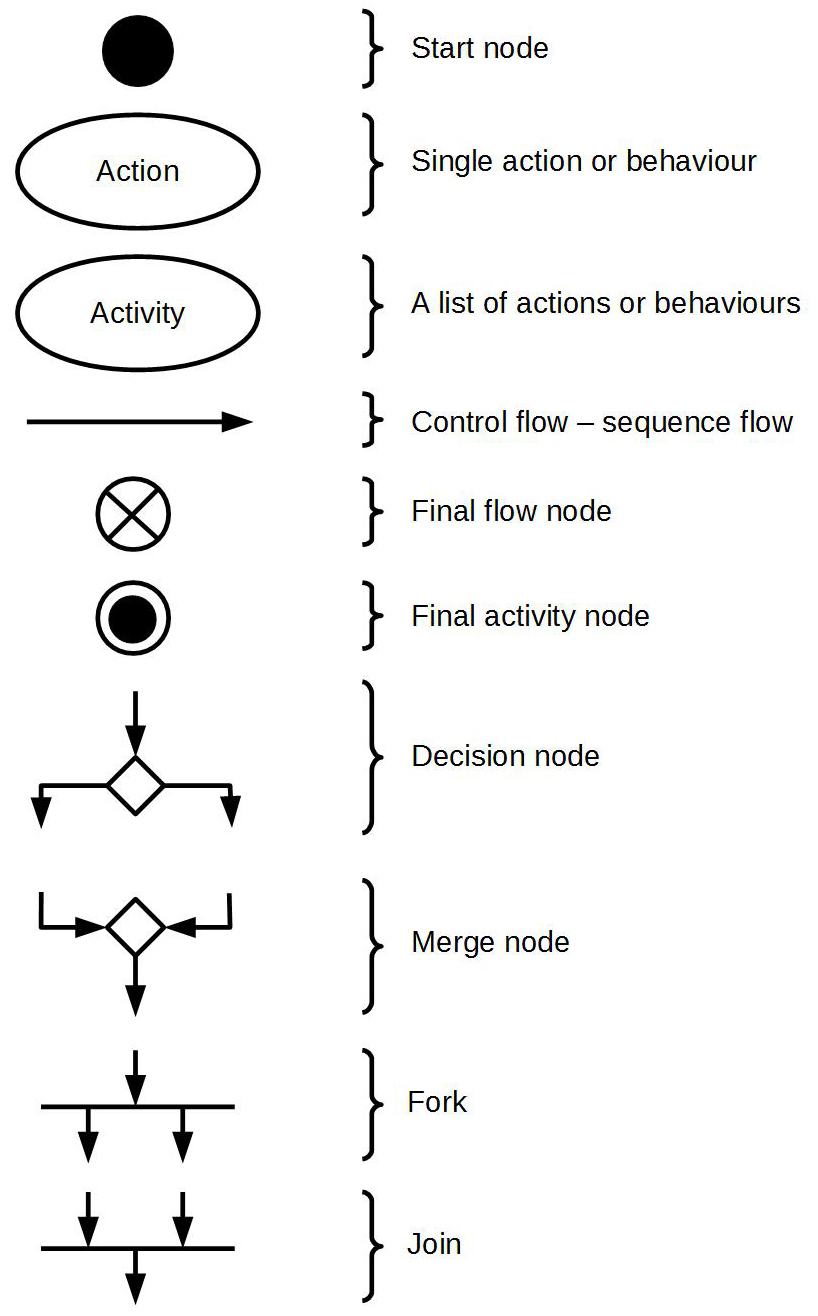
\includegraphics[width=0.75\linewidth]{IDSTEORIA/Immagini/UML/ActivityDiagram.png}
    \caption{Notazione grafica dei vari elementi di un Activity Diagram.}
\end{figure}